% \iffalse
\let\negmedspace\undefined
\let\negthickspace\undefined
\documentclass[journal,12pt,twocolumn]{IEEEtran}
\usepackage{cite}
\usepackage{amsmath,amssymb,amsfonts,amsthm}
\usepackage{algorithmic}
\usepackage{graphicx}
\usepackage{textcomp}
\usepackage{xcolor}
\usepackage{txfonts}
\usepackage{listings}
\usepackage{enumitem}
\usepackage{mathtools}
\usepackage{gensymb}
\usepackage{comment}
\usepackage[breaklinks=true]{hyperref}
\usepackage{tkz-euclide} 
\usepackage{tikz}
% \usetikzlibrary{positioning, arrows.meta}
\usepackage{listings}
\usepackage{gvv} 
\usepackage{caption}
\def\inputGnumericTable{}                   

%\usepackage[latin1]{inputenc}                                
\usepackage{color}                                            
\usepackage{array}                                            
\usepackage{longtable}                                       
\usepackage{calc}                                             
\usepackage{multirow}                                         
\usepackage{hhline}                                           
\usepackage{ifthen}                                           
\usepackage{lscape}
\usepackage{tikz}
\newtheorem{theorem}{Theorem}[section]
\newtheorem{problem}{Problem}
\newtheorem{proposition}{Proposition}[section]
\newtheorem{lemma}{Lemma}[section]
\newtheorem{corollary}[theorem]{Corollary}
\newtheorem{example}{Example}[section]
\newtheorem{definition}[problem]{Definition}
\newcommand{\BEQA}{\begin{eqnarray}}
\newcommand{\EEQA}{\end{eqnarray}}
\newcommand{\define}{\stackrel{\triangle}{=}}
\theoremstyle{remark}
\newtheorem{rem}{Remark}

\begin{document}

\bibliographystyle{IEEEtran}
\vspace{3cm}

\title{GATE: IN - 41.2022}
\author{EE23BTECH11013 - Avyaaz$^{*}$% <-this % stops a space 
}
\maketitle
\newpage
\bigskip

\renewcommand{\thefigure}{\arabic{figure}}
\renewcommand{\thetable}{\arabic{table}}

\large\textbf{\textsl{Question:}}
A proportional-integral-derivative (PID) controller is employed to stably control a
plant with transfer function
\begin{align}
    P(s) = \frac{1}{(s+1)(s+2)}
\end{align}
Now, the proportional gain is increased by a factor of $2$, the integral gain is
increased by a factor of $3$, and the derivative gain is left unchanged. Given that the closed-loop system continues to remain stable with the new gains, the steady-state
error in tracking a ramp reference signal\hfill(GATE IN 2022) \\
\solution

\begin{table}[htbp]
    \centering
     \begin{tabular}{|c|c|c|}
    \hline
    \textbf{Parameter} & \textbf{Description} & \textbf{Value} \\
    \hline
     \(x(0)\) & First Term &\(\dfrac{5}{2}\) \\
    \hline
     \(r\) = \(\dfrac{x(1)}{x(0)}\) & Common Ratio & \(\dfrac{1}{2}\) \\
    \hline
      \(x(n)\) & \(n^{th}\) Term & \(\dfrac{5}{2}\left(\dfrac{1}{2}\right)^n \cdot u(n)\) \\
    \hline
     \(x(19)\) & \(20^{th}\) Term &\(\dfrac{5}{2} \left(\dfrac{1}{2}\right)^{19}\) \\
    \hline
     \(u(n)\) &Unit step function & \\
    \hline
  \end{tabular}

    \caption{Caption}
    \label{tab:my_label}
\end{table}
\noindent The transfer function of PID controller,

\begin{align}
    G_c(s) = K_p + \frac{K_I}{s} +sK_D\\
    =\frac{s^2K_D + sK_P + K_I}{s}
\end{align}
Overall loop-transfer function,
\begin{align}
    L(s) &= G_c(s)\cdot P(s)\\
    L(s) &= \frac{s^2K_D + sK_p + K_I}{s(s+1)(s+2)}
\end{align}
Steady-state error due to ramp signal,
\begin{align}
    e_{ss} = \frac{1}{K_v}
\end{align}
where,
\begin{align}
    K_v = \lim_{s \to 0} sL(s)
\end{align}
\begin{align}
    K_v = \frac{K_I}{2}\\
    e_{ss} = \frac{2}{K_I}
\end{align}
Now, the proportional gain is increased by a factor of 2, the integral gain is increased by a factor of 3, and the derivative gain is left unchanged.
\begin{align}
    K'_P = 2K_P, K'_I = 3K_I \text{ and } K'_D = K_D
\end{align}
\begin{align}
    K'_v = \lim_{s \to 0} sL'(s)\\
    K'_v = \frac{3K_I}{2}\\
    e'_{ss} = \frac{1}{K'_V} = \frac{2}{3K_I}
\end{align}
\begin{figure}[!ht]
    \resizebox{0.55\textwidth}{!}{% \tikzset{
%     block/.style = {draw, fill=white, rectangle, minimum height=3em, minimum width=3em},
%     tmp/.style  = {coordinate}, 
%     minus/.style= {draw, fill=white, circle, node distance=1cm, append after command={\pgfextra \draw ($(\tikzlastnode.center) + (-0.15,0)$) -- ($(\tikzlastnode.center) + (0.15,0)$) node[above] {$-$}; \endpgfextra}},
%     plus/.style= {draw, fill=white, circle, node distance=1cm, append after command={\pgfextra \draw ($(\tikzlastnode.center) + (-0.15,0)$) -- ($(\tikzlastnode.center) + (0.15,0)$) node[above] {$+$}; \endpgfextra}},
%     input/.style = {coordinate},
%     output/.style= {coordinate},
%     pinstyle/.style = {pin edge={to-,thin,black}}
% }


% \begin{tikzpicture}[auto, node distance=2cm,>=latex']
%     \node [input, name=rinput] (rinput) {};
%     \node [minus, right of=rinput] (sum1) {};
    
%     \node [block, right of=sum1] (controller) {$k_{p}$};
%     \node [block, above of=controller, node distance=2cm] (up) {$\frac{k_{i}}{s}$};
%  \node [block, below of=controller, node distance=2cm] (kd) {$K_d$};
 
%     \node [plus, right of=controller, node distance=2cm] (sum2) {};
%     \node [block, right of=sum2, node distance=3.5cm] (system) {$G\brak{s}=\frac{1}{\brak{s-1}}$};
%     \node [output, right of=system, node distance=2cm] (output) {};
%     \node [tmp, below of=controller] (tmp1) {$H(s)$};

%     \draw [->] (rinput) -- node[below]{$r\brak{t}$} (sum1);
%     \draw [->] (sum1) -- node[name=z,anchor=north,fill=white,circle,inner sep=1pt]{$e\brak{t}$} (controller);
%     \draw [->] (controller) -- (sum2);
%     \draw [->] (sum2) -- node[above, pos=0.8]{$w\brak{t}$} (system);
%     \draw [->] (system) -- node [name=y] {$y\brak{t}$} (output);
%     \draw [->] (z) |- (up);
%     \draw [->] (up) -| (sum2);
%     % \draw [->] (y) |- (tmp1) -| (sum1);
% \end{tikzpicture}



% \begin{tikzpicture}[auto, node distance=2cm,>=latex']
%     \node [input, name=rinput] (rinput) {};
%     \node [minus, right of=rinput] (sum1) {};
    
%     \node [block, right of=sum1] (controller) {$k_{p}$};
%     \node [block, above of=controller, node distance=2cm] (up) {$\frac{k_{i}}{s}$};
%     \node [block, below of=controller, node distance=2cm] (kd) {$K_d$};
 
%     \node [plus, right of=controller, node distance=2cm] (sum2) {};
%     \node [block, right of=sum2, node distance=3.5cm] (system) {$G\brak{s}=\frac{1}{\brak{s-1}}$};
%     \node [output, right of=system, node distance=2cm] (output) {};
%     \node [tmp, below of=controller] (tmp1) {$H(s)$};

%     \draw [->] (rinput) -- node[below]{$r\brak{t}$} (sum1);
%     \draw [->] (sum1) -- node[name=z,anchor=north,fill=white,circle,inner sep=1pt]{$e\brak{t}$} (controller);
%     \draw [->] (controller) -- (sum2);
%     \draw [->] (sum2) -- node[above, pos=0.8]{$w\brak{t}$} (system);
%     \draw [->] (system) -- node [name=y] {$y\brak{t}$} (output);
%     \draw [->] (z) |- (up);
%     \draw [->] (up) -| (sum2);
%     \draw [->] (z) |- (kd);
%     \draw [->] (kd) -| (sum2);
%     \draw [->] (y) |- (tmp1) -| (sum1);
% \end{tikzpicture}

\begin{tikzpicture}[auto, node distance=2cm,>=latex']
    % Blocks
    \node [input, name=rinput] (rinput) at (0,0) {};
    \node [minus] (sum1) at (1,0) {};
    \node [block] (controller) at (3,0) {$K_{p}$};
    \node [block] (kd) at (3,-2) {$sK_D$};
    \node [block] (up) at (3,2) {\Large$\frac{K_{i}}{s}$};
    \node [plus] (sum2) at (5,0) {};
    \node [block] (system) at (7,0) {$P\brak{s}=\frac{1}{\brak{s+1}\brak{s+2}}$};
    \node [output] (output) at (9,0) {};
    \node [tmp] (tmp1) at (3,-4) {$H(s)$};

    % Connectors
    \draw [->] (rinput) -- node[below]{$r\brak{t}$} (sum1);
    \draw [->] (sum1) -- node[name=z,anchor=north,fill=white,circle,inner sep=1pt]{$e\brak{t}$} (controller);
    \draw [->] (controller) -- (sum2);
    \draw [->] (sum2) -- node[above, pos=-2.5]{$G_c\brak{t}$} (system);
    \draw [->] (system) -- node [pos = 1,name=y] {$L\brak{t}$} (output);
    \draw [->] (z) |- (up);
    \draw [->] (up) -| (sum2);
    \draw [->] (z) |- (kd);
    \draw [->] (kd) -| (sum2);
    \draw [->] (y) |- (tmp1);
    \draw [->] (tmp1) -| (sum1);
\end{tikzpicture}
}
    \caption{Block Diagram of System}
    \label{fig:gate_IN_Q41_blockdiagram}
\end{figure}

\begin{figure}[htbp]
    \centering
    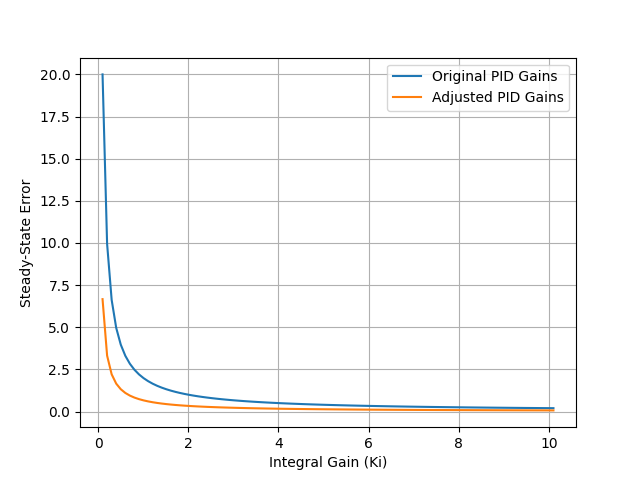
\includegraphics[width = \columnwidth]{figs/steady_state_error.png}
  \caption{}
    \label{fig:graph1.41.IN.2022}
\end{figure}

% \begin{figure}[htbp]
%     \centering
%     \includegraphics[width = \columnwidth]{}
%   \caption{}
%     \label{fig:graph1}
% \end{figure}

% \bibliographystyle{IEEEtran}
\end{document}
